%%%%%%%%%%%%%%%%%%%%%%%%%%%%%%%%%%%%%%%%%
% Arsclassica Article
% LaTeX Template
% Version 1.1 (10/6/14)
%
% This template has been downloaded from:
% http://www.LaTeXTemplates.com
%
% Original author:
% Lorenzo Pantieri (http://www.lorenzopantieri.net) with extensive modifications by:
% Vel (vel@latextemplates.com)
%
% License:
% CC BY-NC-SA 3.0 (http://creativecommons.org/licenses/by-nc-sa/3.0/)
%
%%%%%%%%%%%%%%%%%%%%%%%%%%%%%%%%%%%%%%%%%

%----------------------------------------------------------------------------------------
%	PACKAGES AND OTHER DOCUMENT CONFIGURATIONS
%----------------------------------------------------------------------------------------

\documentclass[
article,
10pt, % Main document font size
oneside, % One page layout (no page indentation)
BCOR5mm, % Binding correction
]{scrartcl}
\usepackage[a4paper,margin=3cm]{geometry}
\usepackage[italian]{babel}
\usepackage[utf8]{inputenc}
\usepackage{atbegshi}% http://ctan.org/pkg/atbegshi
\usepackage{tikz}
\usetikzlibrary{shapes}
\usepackage{amsmath}
\usepackage{xspace}
\usepackage[usestackEOL]{stackengine}
\usepackage{graphicx}
\usepackage{caption}
\usepackage{subcaption}
\usepackage{float}
\newcommand{\A}{\ensuremath{\mathcal{A}}\xspace}
\newcommand{\B}{\ensuremath{\mathcal{B}}\xspace}
\newcommand\pa[1]{\ensuremath{\left(#1\right)}}
\AtBeginDocument{\AtBeginShipoutNext{\AtBeginShipoutDiscard}}

\hyphenation{Fortran hy-phen-ation} % Specify custom hyphenation points in words with dashes where you would like hyphenation to occur, or alternatively, don't put any dashes in a word to stop hyphenation altogether

%----------------------------------------------------------------------------------------
%	TITLE AND AUTHOR(S)
%----------------------------------------------------------------------------------------

\begin{document}

\begin{center}
\title{
  \begin{figure}[h!]
  \centering
  
\includegraphics{images/icona_titolo.png}
  \end{figure}
  Valutazione dell'accessibilità del sito \\
  Libreria di Valyria
}
\author{Carlo Munarini 1050128 \\
Sebastiano Valle 1050123}
\end{center} % The article author(s) - author affiliations need to be specified in the AUTHOR AFFILIATIONS block






%\date{} % An optional date to appear under the author(s)

%----------------------------------------------------------------------------------------

%----------------------------------------------------------------------------------------
%	TABLE OF CONTENTS & LISTS OF FIGURES AND TABLES
%----------------------------------------------------------------------------------------

\maketitle % Print the title/author/date block

\setcounter{page}{1} % Set the depth of the table of contents to show sections and subsections only

{\raggedleft\vfill\Longstack[l]{%
Indirizzo: \texttt{http://tecnologie-web.studenti.math.unipd.it/tecweb/$\sim$aongaro} \\
Email referente: \texttt{sebastiano.valle@hotmail.it}
}
\raggedright{}
\newpage{}
\tableofcontents % Print the table of contents



\listoffigures % Print the list of figures

\listoftables % Print the list of tables

\section{Struttura}
Di seguito sono illustrate le modalità di progettazione della struttura delle
pagine all'interno del sito.

\subsection{Parti comuni a tutte le pagine}
Tutte le pagine sono state scritte seguendo lo standard \textit{XHTML 1.0 Strict} e come codifica è stata scelta UTF-8 dal momento che nel sito sono
presenti parole accentate.
Una sezione \textbf{head} ed una sezione \textbf{body} sono state inserite in
tutte le pagine con la stessa struttura.

\subsubsection{Head} %TODO @Graziano @Carlo
Sono presenti i seguenti tag nelle sezioni head di tutte le pagine:
\begin{itemize}
\item \textbf{title:} permette di visualizzare sulla finestra del browser il titolo della pagina visualizzata, dal particolare al generale
\item \textbf{meta title:} indica il titolo della pagina in un eventuale snippet, anch'esso dal particolare al generale
\item \textbf{meta description:} in questo tag viene inserita la breve descrizione della pagina visualizzata in un eventuale snippet
\item \textbf{meta author:} in questo tag sono indicati i componenti del gruppo
\item \textbf{meta keywords:} parole che aiutano un motore di ricerca a trovare la pagina grazie a dei termini di importanza focale
\item \textbf{meta robots:} tag che indica ad un eventuale spider se indicizzare la pagina e se seguire i link da essa uscenti
\item \textbf{meta keywords:} parole che aiutano un motore di ricerca a trovare la pagina grazie a dei termini di importanza focale
\item \textbf{meta reply-to:} %TODO@Graziano
\item \textbf{meta Classification:} tag che serve ad indicare l'argomento trattato dalle pagine del sito
\item \textbf{meta viewport:} %TODO@Carlo
\item \textbf{link shortcut icon:} icona visibile a fianco al titolo della scheda nel browser, aiuta a identificare meglio le schede di \textit{What To Visit} se un utente avesse più schede aperte nel suo browser
\item \textbf{link stylesheet:} collegamento a foglio di stile CSS %TODO@Carlo
\end{itemize}

\subsubsection{Body}
Affinchè l'utente si sentisse il meno disorientato possibile all'interno di \textit{What To Visit}, si è cercato di progettare il sito con un layout essenziale e che mettesse in primo piano il contenuto aspettato in tutte le pagine.
Sono presenti questi elementi strutturali nei corpi di tutte le pagine:
\begin{itemize}
\item un header, dove vi è il logo del sito;
\item un'ampia parte centrale, dove vengono visualizzati i contenuti richiesti dall'utente;
\item un footer, dove sono presenti link ed informazioni di poco rilievo e un'indicazione riguardo la validità della pagina.
\end{itemize}

\subsection{Homepage}
Come pagina principale del sito, si è pensato di esporre in primo piano all'utente la scelta delle tre categorie delle località.
A partire da queste l'utente può arrivare nelle pagine delle categorie, dove può trovare le liste delle località presenti in queste.

Dal momento che la homepage è l'unica pagina facilmente riconoscibile data la sua struttura con tre titoli di indirizzamento, la breadcrumb è stata omessa perchè si è assunto che gli utenti riuscissero a dedurre che si trovano nella homepage quando vi sono dentro (anche grazie all'URL).

Per poter comunque fornire collegamenti alle pagine che non sono di contenuto ma che sono significative (Chi Siamo e F.A.Q.), i link a queste sono stati inseriti nell'header della pagina a fianco del logo; in questo modo, anche se sono di importanza secondaria rispetto ai tre pannelli visualizzati nella pagina, rimangono comunque nella parte visibile del sito quando questo viene aperto (\texttt{http://en.wikipedia.org/wiki/Above\_the\_fold\#In\_web\_design}).

Nel footer, oltre alle indicazioni di validità della pagina, sono stati lasciati i link restanti alle pagine che non sono di contenuto.
 % 80%

\section{Schema organizzativo}\label{sec:schema-org}
Lo schema organizzativo del sito è chiaramente ambiguo:
\begin{itemize}
\item Non ci sono abbastanza informazioni per determinare se un libro nella
sezione ``nuovi" della home sia un libro uscito pubblicamente di recente o un
libro appena arrivato nella collezione della libreria;
\item Nella sezione ``più votati" nella home non è possibile sapere se
l'utente troverà lo stesso libro in tale sezione in due visite compiute in
momenti differiti;
\item Nella sezione ``Generi", un libro potrebbe appartenere a due categorie
diverse (ad esempio ci si aspettava di trovare \textit{Divergent} in
``Narrativa");
\item Nella sezione ``Generi", dopo la selezione del genere non è chiaro
l'ordine in cui sono visualizzati i libri;
\item La ricerca, per come è presentata, farebbe pensare ad uno schema
organizzativo; tuttavia, si parlerà più in dettaglio di ciò nella sezione
seguente ed è doverso notare che non sempre fornisce i risultati attesi (ad
esempio eseguendo la ricerca per autore e immettendo la lettera \'r\' viene
mostrato solamente un libro di Glenn Cooper).
\end{itemize}

In particolare, la ricerca per collana è ambigua perchè non vi sono
indicazioni su come svolgere la ricerca: l'utente quindi non sa cosa può
inserire precisamente in tale campo per effettuare la ricerca.

\subsection{Elenchi di libri}\label{sec:schema-elenchi}
Dopo varie ricerche e dopo aver esplorato tutti i generi letterari offerti, ai
verificatori è parso che i libri in questi elenchi siano visualizzati secondo
l'ordine cronologico di apparizione nella libreria, dal più vecchio al
più recente. Tuttavia questa scelta sembra poco plausibile poichè si ritiene
che gli utenti siano interessati alle opere più nuove, come la selezione dei
sei titoli proposta in home.

Per questo motivo si ritiene che manchi del tutto uno schema organizzativo e
che l'ordine trovato nella generazione degli elenchi sia \textbf{incidentale},
mentre sarebbe sufficiente uno schema organizzativo esatto che rispetta
l'ordine alfabetico (o presentando i libri dal più recente al meno recente,
evidenziando la data di pubblicazione/inserimento) per poter aiutare l'utente
nell'esplorazione del sito. % 70%

\section{Accessibilità}\label{sec:accessibilita}
Nel sito non è stato indicato nessuno standard di accessibilità raggiunto.
Tramite un analisi, si è notato inoltre che non vengono soddisfatte nè le
richieste di WAI-A WCAG2.0 nè della ``section 508".
Di seguito verranno infatti descritte le mancanze rilevate nel sito in termini
di accessibilità, ordinate secondo le 14 linee guida di WAI; dove non conforme,
verrà indicato la priorità del punto di controllo dove è stata riscontrata la
mancanza.

\subsection{Linee guida per l'accessibilità}

\subsubsection{Fornire alternative equivalenti al contenuto audio e visivo}
\begin{enumerate}
\item Non sempre viene fornito un equivalente testuale per gli elementi non
testuali, ad esempio nella pagina principale mancano gli attributi \texttt{alt}
ai tag \texttt{img}
(\textit{Priorità 1});
\item Non sono presenti mappe immagine, perciò 1.2 è rispettato;
\item Non sono presenti filmati, perciò 1.3 è rispettato;
\item Non sono presenti filmati, perciò 1.4 è rispettato;
\item Non sono presenti mappe immagine, perciò 1.5 è rispettato.
\end{enumerate}

Il punto di controllo 1.1 fallisce e questo è sufficiente per dire che la
pagina non è accessibile per WAI-A WCAG2.0. Di seguito non verrà più
evidenziato tale fatto (nemmeno per i gradi successivi di accessibilità) poichè
il non-rispetto di un solo punto di controllo compromette il grado complessivo
di accessibilità del sito.

\subsubsection{Non fare affidamento sul solo colore}
\begin{enumerate}
\item L'informazione arriva tramite indicazioni indipendenti dal colore;
\item Il contrasto è abbastanza marcato da poter permettere una corretta visualizzazione del sito e, anche nel caso di mancanto caricamento delle immagini di sfondo, sono stati utilizzati degli accorgimenti che garantiscono una visualizzazione decente di alcuni elementi come i titoli/intestazioni.
\end{enumerate}

\subsubsection{Usare marcatori e fogli di stile e farlo in modo appropriato}
\begin{enumerate}
\item Le pagine sono scritte secondo lo standard \textbf{XHTML 1.0 Strict},
sebbene poi non sempre venga rispettato;
\item Tutte le pagine si riferiscono correttamente allo schema \textbf{DTD} di
XHTML 1.0 Strict;
\item Il tag \textit{hr} è utilizzato per meri scopi presentazionali, ovvero
l'inserire un bordo tra delle intestazioni e il contenuto sottostante (ad
esempio in \texttt{about.html}); oltre a questo, sono talvolta inseriti
\texttt{span} per puro scopo presentazionale e non semantico, come quello in
\texttt{\#path} (\textit{Priorità 2});
\item Vengono utilizzate delle unità assolute come \texttt{font-size: medium}
per il testo (\textit{Priorità 2});
\item Gli elementi di intestazione sono usati correttamente, tuttavia si
potrebbe pensare di inserirne altri per favorire la lettura del contenuto da
parte di screen-reader o altri dispositivi che fanno molto affidamento sulle
intestazioni;
\item Vi sono alcune \texttt{dl} che vengono scritte però marcate come
\texttt{ul}, comportando l'aggiunta di tag come \texttt{strong} a parti
dell'item listato per emulare i tag \texttt{dt} e \texttt{dd}
(\textit{Priorità 2});
\item Non sono presenti citazioni, perciò 3.7 è rispettato.
\end{enumerate}

\subsubsection{Chiarire l'uso di linguaggi naturali}
\begin{enumerate}
\item Non viene mai segnalato il cambio linguaggio, ad esempio \textit{home} o
\textit{user} in \texttt{accesso.html} (\textit{Priorità 1});
\item Non vengono mai segnalate abbreviazioni, ad esempio \textit{LDV} in
qualsiasi pagina di un libro o ``\textit{J.K. Rowling}" in
\texttt{ricerca.html} (\textit{Priorità 3});
\item Viene correttamente identificato il linguaggio del documento, perciò 4.3
è rispettato.
\end{enumerate}

\subsubsection{Creare tabelle che si trasformino in maniera elegante}
\begin{enumerate}
\item Non sono presenti tabelle, perciò 5.1 è rispettato;
\item Non sono presenti tabelle, perciò 5.2 è rispettato;
\item Non sono presenti tabelle, perciò 5.3 è rispettato;
\item Non sono presenti tabelle, perciò 5.4 è rispettato;
\item Non sono presenti tabelle, perciò 5.5 è rispettato;
\item Non sono presenti tabelle, perciò 5.6 è rispettato.
\end{enumerate}

\subsubsection{Assicurarsi che le pagine che danno spazio a nuove tecnologie
si trasformino in maniera elegante}
\begin{enumerate}
\item Il contenuto, seppur presentando errori di markup, è sufficientemente
leggibile e comprensibile senza fogli di stile, perciò 6.1 si può ritenere
rispettato;
\item Non si ritiene che i contenuti dinamici del sito possano essere
modificati una volta inseriti, se non per i commenti in coda ai libri;
tuttavia l'aggiornamento automatico tramite AJAX o altre tecnologie esulava
dagli obiettivi del corso di Tecnologie Web, perciò 6.2 si può ritenere
rispettato;
\item Le pagine perdono gran parte della loro usabilità disattivando
JavaScript, ad esempio ogni form, anzichè avere un input di tipo
\textbf{submit}, gestisce la sottomissione dei dati inseriti via JavaScript
con un input di tipo \textbf{button}, compromettendo normali operazioni che
sarebbero possibili utilizzando nella struttura i tag semanticamente corretti
(\textit{Priorità 1});
\item I gestori degli eventi non dipendono da particolari dispositivi che
utilizzano JavaScript, perciò 6.4 è rispettato;
\item Le pagine che non risultano accessibili disattivando JavaScript non
forniscono alcuna pagina o presentazione alternativa (\textit{Priorità 2}).
\end{enumerate}

\subsubsection{Assicurarsi che l'utente possa tenere sotto controllo i
cambiamenti di contenuto nel corso del tempo}
\begin{enumerate}
\item Nessun componente nella pagina causa fenomeni di sfarfallio, perciò 7.1
è rispettato;
\item Nessun componente nella pagina causa fenomeni di lampeggiamento, perciò
7.2 è rispettato;
\item Nessun componente nella pagina si muove una volta caricato, perciò 7.3 è
rispettato;
\item Le pagine non si aggiornano automaticamente, perciò 7.4 è rispettato;
\item Non vi sono pagine che effettuano auto-reindirizzamento, perciò 7.5 è
rispettato.
\end{enumerate}

\subsubsection{Assicurare l'accessibilità diretta delle interfacce utente
incorporate}
\begin{enumerate}
\item Gli script sono ritenuti accessibili verso i dispositivi che li
supportano, perciò 8.1 è rispettato.
\end{enumerate}

\subsubsection{Progettare per garantire l'indipendenza da dispositivo}
\begin{enumerate}
\item Non sono presenti mappe immagine, perciò 9.1 è rispettato;
\item Ogni elemento è accessibile indipendemente dal dispositivo con cui si
naviga nel sito, perciò 9.2 è rispettato;
\item Gli eventi si riferiscono a gesture o actions astratte o logiche e non
relative a specifici dispositivi, perciò 9.3 è rispettato;
\item Non è specificato un ordine di tabulazione diverso da quello di default,
sebbene potrebbe essere utile in questo sito (\textit{Priorità 3});
\item Non sono definite scorciatoie da tastiera, il che potrebbe essere
positivo o negativo a seconda delle motivazioni che risiedono dietro questa
scelta; 9.5 si può ritenere rispettato.
\end{enumerate}

\subsubsection{Usare soluzioni provvisorie}
\begin{enumerate}
\item La finestra attiva non viene mai cambiata nè vengono generate nuove
finestre nè appaiono finestre a cascata, perciò 10.1 è rispettato;
\item Sebbene le label degli input nei form siano associate in modo erroneo
(come discusso nella sezione \ref{sec:acc-form}), queste sono posizionate
correttamente a livello presentazionale rispetto ai rispettivi input, perciò
10.2 è rispettato;
\item Non ci sono tabelle, perciò 10.3 è rispettato;
\item I placeholder ci sono, ma non sempre funzionano nel modo aspettato (come
discusso nella sezione \ref{sec:acc-form}) (\textit{Priorità 3});
\item Non sono presenti molti link nelle pagine e nessuno di questi è
adiacente a un altro senza altri elementi o tag tra i due link, perciò 10.5 è
rispettato.
\end{enumerate}

\subsubsection{Usare le tecnologie e le raccomandazioni del W3C}
\begin{enumerate}
\item Vengono utilizzate solamente tecnologie W3C (anche se talvolta non
rispettando gli standard), perciò 11.1 è rispettato;
\item Le label dei form sono associate al contenuto degli attributi
\texttt{name} (come detto nella sezione \ref{sec:acc-form}) e non a quello
degli attributi \texttt{id}, come da raccomandazione W3C; essendo pratica non
prevista dall'ente, presumibilmente è anche disapprovata
(\textit{Priorità 2});
\item Non si vedono nè localizzazione nè globalizzazione come prospettive di
tale sito, perciò 11.3 è rispettato;
\item Durante la realizzazione del sito probabilmente non è stato notato che
le pagine non rispettano gli standard o che presentano problemi di
accessibilità, perciò non sono fornite versioni alternative
\textit{accessibili} delle pagine del sito (\textit{Priorità 1}).
\end{enumerate}

\subsubsection{Fornire informazione per la contestualizzazione e
l'orientamento}
\begin{enumerate}
\item Non sono presenti \textbf{frame}, perciò 12.1 è rispettato;
\item Non sono presenti frame, perciò 12.2 è rispettato;
\item I campi delle form sono raggruppati con tag \texttt{fieldset} e
\texttt{legend}, perciò 12.3 è rispettato;
\item Come descritto nella sezione \ref{sec:acc-form}, i tag \texttt{label}
non sono associati agli input correttamente (\textit{Priorità 2}).
\end{enumerate}

\subsubsection{Fornire chiari meccanismi di navigazione}
\begin{enumerate}
\item I link fanno effettivamente capire dove portano, ma mancano gli
attributi \texttt{title} per spiegare meglio cosa riferisce l'ancora, perciò
13.1 si può ritenere rispettato in modo lasco;
\item L'utilizzo dei meta tag è sempre scorretto, poichè i contenuti dei pochi
tag presenti sembrano presi da un template XHTML (ad esempio in
\texttt{about.html} il tag \texttt{description} ha come contenuto
\textit{Inserisci le descrizioni}) e mancano tag importanti, come
\texttt{author} (\textit{Priorità 2});
\item Non è presente nessuna pagina dedicata all'orientamento sul sito, nè
mappa nè un indice ben definito (non è presente nemmeno una \textit{sitemap}
\footnote{\texttt{https://support.google.com/webmasters/answer/183668?hl=it}}
vera e propria), non rispettando di fatto il punto di controllo 13.3
(\textit{Priorità 2});
\item Come descritto nella sezione \ref{sec:user-ui_consistency}, gli elementi
di navigazione non sono consistenti o coerenti nelle varie pagine del sito
(\textit{Priorità 2});
\item Il sito non dispone sempre di una barra di navigazione, ad esempio nella
pagina visualizzata se si fallisce l'accesso (\textit{Priorità 3});
\item Il sito non ha necessità di forkare codice per diversi
\textit{user agent}, perciò 13.6 è ritenuto rispettato;
\item Il sito offre diversi metodi di ricerca (sebbene questa non funzioni
correttamente come descritto nella sezione \ref{sec:schema-org}), perciò 13.7
è rispettato;
\item In alcune parti l'informazione più significativa non è posta all'inizio
di elenchi, come descritto nella sezione \ref{sec:schema-elenchi}
(\textit{Priorità 3});
\item Non sono presenti documenti composti da più pagine, perciò 13.9 è
rispettato;
\item Non sono presenti immagini realizzate con l'\textit{ASCII multi-line}
\footnote{\texttt{https://trendimpulse.wordpress.com/tag/multiple-lines-ascii-art/}}, perciò 13.10 è rispettato.
\end{enumerate}

\subsubsection{Assicurarsi che i documenti siano chiari e semplici}
\begin{enumerate}
\item Anche se il testo non sempre è grammaticalmente corretto e semplice, si
ritiene che la (\textbf{seconda}) scelta sia dovuta al fatto che l'audience è
un pubblico di cultura letteraria medio-alta (essendo il sito di una
biblioteca), perciò 14.1 si può ritenere rispettato;
\item Sono mostrate le immagini delle copertine dei libri, mentre l'audio
potrebbe essere meno significativo per aumentare il valore del contenuto,
perciò 14.2 è rispettato;
\item Lo stile di presentazione è comune a tutte le pagine, perciò 14.3 è
rispettato.
\end{enumerate}

%%%%%% FINE LINEE GUIDA -> QUI SI METTONO TUTTE LE COSE NON SALTATE FUORI PRIMA

\subsection{Errori non risultati dal confronto con le linee guida}

\subsubsection{Form}\label{sec:acc-form}
I form presentano vari errori:
\begin{itemize}
\item I form sono spesso bizzarramente contrassegnati con la classe
\texttt{forms}, come in \texttt{ricerca.html}, rompendo nuovamente la
separazione presentazione-struttura;
\item Non compaiono gli input di submit, rendendo impossibile la richiesta di
azione di un form se JavaScript è disattivato (si ritiene che non siano stati
messi i submit poichè fosse lievemente più complesso gestire l'arresto
nell'invio della richiesta di sottomissione nel caso in cui i dati inseriti
fossero scorretti, rompendo la separazione comportamento-struttura);
\item Per qualche strano motivo gli input presentano attributi \texttt{name} e
\texttt{id} con contenuto differente;
\item Le label sono associate erroneamente, per cui la pressione sull'elemento
individuato dal tag label non risulta nell'acquisizione del focus sull'input
desiderato;
\item Le ricerche di libri per autore, titolo e collana vengono eseguite con
una chiamata REST di tipo POST, impedendo all'utente di salvare come possibile
segnalibro (una \textbf{boa}, nella \textit{metafora della pesca}) la pagina
contenente i risultati della ricerca effettuata;
\item I placeholder non hanno comportamento del tutto aspettato dall'utente,
dal momento che se l'input perde il focus dopo averlo acquisito ed è vuoto,
non ricompare il placeholder.
\end{itemize}

\subsubsection{Separazione tra elementi del sito}
Qui di seguito vengono evidenziate le incongruenze non precedentemente
segnalate, rispetto alla separazione tra i tre elementi che lo compongono,
ovvero \textbf{struttura}, \textbf{presentazione} e \textbf{comportamento}.

\paragraph{Separazione struttura-comportamento} ~\\
In quasi tutte le pagine HTML c'è codice JavaScript, rompendo in modo netto la
separazione struttura-comportamento.

\paragraph{Separazione struttura-presentazione} ~\\
Alcune classi, come \textit{shiftsx} in \texttt{contatti.html} forniscono
informazioni di carattere presentazionale e non semantico.

Nei form è inserito il tag \texttt{br} a scopo presentazionale, poichè serve
solamente per controllare la posizione del fieldset.

Nella pagina \texttt{registrazione.html} il tag \texttt{br} è usato per far
andare a capo il testo.

Nella pagina \texttt{registrazione.html} è associata la classe
\textit{link\_blok} che presuppone che il link sia visualizzato all'interno di
un proprio blocco, ma ciò non avviene. Il nome della classe non ha carattere
semantico ma presentazionale.

Come in \texttt{generi.html}, sono state inserite classi non necessarie per
modificare l'aspetto presentazionale di elementi (le classi
\textit{adattaicona} associate ai link).

\paragraph{Separazione presentazione-comportamento} ~\\
In \texttt{registration\_control.js}, viene assegnato esplicitamente il colore
di elementi tramite JavaScript (con l'attributo \texttt{style}, inserendo CSS
inline).
 % 0%

%%%%%%%%%%%%%%%%%%%%%%%%%%%%%%%
% FONT SCELTO
% TALVOLTA POCO LEGGIBILE (E.G. TITOLI)
%%%%%%%%%%%%%%%%%%%%%%%%%%%%%%%

%%%%%%%%%%%%%%%%%%%%%%%%%%%%%%%
% ALT/TITLE
% NON SEMPRE PRESENTI
%%%%%%%%%%%%%%%%%%%%%%%%%%%%%%%

%%%%%%%%%%%%%%%%%%%%%%%%%%%%%%%
% NON VEDO/NON SENTO
% PROVARE LA PAGINA CON VISCHECK
% PROVARE LA PAGINA CON FANGS
%%%%%%%%%%%%%%%%%%%%%%%%%%%%%%%

%%%%%%%%%%%%%%%%%%%%%%%%%%%%%%%
% B/W
% TESTARE LA PAGINA IN BIANCO E NERO
%%%%%%%%%%%%%%%%%%%%%%%%%%%%%%%

%%%%%%%%%%%%%%%%%%%%%%%%%%%%%%%
% META TAG
% DESCRIZIONI E CONTENUTI SONO PROBABILMENTE PRESI DA UN TEMPLATE
%%%%%%%%%%%%%%%%%%%%%%%%%%%%%%%

\section{Esperienza utente}\label{sec:user-exp}
Di seguito vengono riportate le considerazioni riguardo la qualità del sito in
termini di \textbf{user experience}.

\subsection{Consistenza dell'interfaccia}\label{sec:user-ui_consistency}
L'interfaccia è consistente e utilizza sempre gli stessi elementi grafici per
denotare elementi comuni a diverse pagine, eccezion fatta per:
\begin{itemize}
\item il blocco di navigazione \textbf{non} presente in tutte le pagine;
\item i link in \texttt{accesso.html} e \texttt{registrazione.html};
\item la breadcrumb (in tali pagine contrassegnata con l'id \texttt{path}) non
sempre è strutturata nello stesso modo, contenendo una o due voci a seconda
dei casi (e.g. in \texttt{about.html} e nella pagina generata dalla ricerca);
\item l'utente per poter inserire un commento (e quindi completare un task
relativo alla pagina dove è descritto un libro) deve accedere ad una nuova
pagina per scrivere il commento, senza che in questa nuova pagina siano
visualizzate le informazioni sul libro.
\end{itemize}

Sebbene presenti i problemi sopra descritti, l'interfaccia è comunque ritenuta
consistente rispetto al contesto in cui è inserita (una libreria) e alle
medie aspettative che un utente avrebbe sapendo di visitare un sito di una
libreria.

\subsection{Area visibile}
Ogni pagina ha un'ampia intestazione che occupa una buona parte di spazio;
tuttavia, non riducendo la pagina a dimensioni eccessivamente ridotte, il
contenuto principale rimane parzialmente visibile (se non questi, almeno i
titoli del contenuto).

Nelle descrizioni dei libri i commenti occupano una posizione di fondo.
Probabilmente i commenti dovrebbero trovare uno spazio nell'area visibile
(\textit{above the fold}). Se non venissero inseriti in questa zona della
pagina, servirebbe almeno un pulsante o un'ancora presente \textit{above the
fold} per poter raggiungere facilmente la sezione della pagina riservata ai
commenti.

\subsection{Informazioni utili}
L'utente non sempre dispone di informazioni accessorie ma utili durante la sua
navigazione: di seguito verranno discusse la loro presenza e, se presenti, le
modalità con cui queste sono state realizzate.

\subsubsection{Informazioni sulla propria posizione}\label{sec:user-posiz}
L'utente se si trova nelle pagine \texttt{accesso.html}, \texttt{logout.html},
\texttt{access\_failure.html} o \texttt{registrazione.html} non dispone di un
blocco di navigazione presente nelle altre pagine.

L'utente non dispone di sufficienti informazioni sulla barra contestuale
(\textit{path} o \textit{breadcrumb}) per capire in che modo ha raggiunto la
pagina in cui si trova. Questa è composta solamente da una voce in quasi tutte
le pagine e, dove non è così, sono visualizzati solamente due livelli di
gerarchia e non il completo percorso dalla home fino alla pagina in questione.

I titoli sono brevi e dal particolare al generale; tuttavia presentano i
seguenti vizi di forma:
\begin{enumerate}
\item I titoli delle pagine hanno l'iniziale minuscola e si ritiene che non sia
una scelta effettuata ma un incidente durante la realizzazione delle pagine;
\item La pagina \texttt{accesso.html} ha come titolo ``acceso";
\item La pagina a cui si accede scegliendo un genere letterario ha come titolo
``risultati". Tale titolo non informa sul contenuto presente nella pagina ed è
una forzatura dal punto di vista semantico; oltre a ciò, è un doppione perchè
vi è un'altra pagina (quella dei risultati di una ricerca) che presenta lo
stesso titolo ma offre funzionalità diverse.
\end{enumerate}

\subsubsection{Pagine di aiuto}
Il sito presenta le pagine ``Chi siamo" e ``Contatti", ma mancano:
\begin{itemize}
\item Una pagina dedicata a (ipotetiche) domande frequenti;
\item Una mappa del sito;
\item Una pagina dove viene illustrata la normativa sulla privacy, dal momento
che il sito raccoglie dati sensibili come indirizzi e-mail.
\end{itemize}

\subsection{Considerazioni di carattere generico}
Sono stati riscontrati i seguenti punti che compromettono gravemente
l'esperienza utente:
\begin{itemize}
\item Link circolare in \texttt{accesso.html} presente in \texttt{\#acces};
\item Difficoltà nell'accedere a funzionalità per utenti autenticati e nel
comprenderle (sezione \ref{sec:user-login});
\item A parte in home (dove è giusto che non sia un link, altrimenti sarebbe
circolare), il logo posto come intestazione principale del sito non è
cliccabile nelle altre pagine del sito, come invece ci si aspetterebbe.
\end{itemize}

\subsubsection{Accesso utente}\label{sec:user-login}
L'accesso utente non viene giustificato in nessuna parte del sito, quindi un
utente deve capire da solo a cosa serve effettivamente registrarsi ed accedere
al sito.

Questo è difficile perchè l'utente deve essere loggato per inserire commenti,
tuttavia la possibilità di effettuare login/registrazione gli viene nascosta
quando si trova nelle sezioni (e.g. pagine del libro, pagine dei generi) dove
effettivamente serve effettuare l'accesso per accedere alle funzionalità.

Da questo deriva naturalmente il fatto che una volta compreso il meccanismo di
come funziona una tipica sessione utente, se questi riaccede al sito per
inserire un commento, non trova il pulsante ``ACCEDI" nelle pagine dove è più
utile, ovvero le pagine che contengono la descrizione di libri.
 % 0%

\section{Test effettuati} %TODO Graziano, Federica, Carlo i test effettuati da voi
In questa sezione si elencano i test effettuati per il sito in esame.
Per i test di accessibilità eseguiti in remoto, il sito è stato caricato su
GitHub Pages.

\subsection{Validazione XHTML} %DONE
Ogni pagina è stata validata con il tool offerto da W3C all'indirizzo
\texttt{http://validator.w3.org/\#validate\_by\_uri}, con il risultato che
le seguenti pagine non sono valide:
\begin{enumerate}
\item pagina principale del sito;
\item pagina descrittiva di un libro (generata tramite CGI).
\end{enumerate}

\subsection{Validazione CSS} %DONE
Ogni foglio di stile CSS è stato validato con il tool offerto da W3C
all'indirizzo
\texttt{https://jigsaw.w3.org/css-validator/\#validate\_by\_input}, non
trovando alcuna scorrettezza nel codice.

\subsection{Cynthia Says} %DONE
Uno dei tool che è stato utilizzato per l'accessibilità delle pagine è Cynthia
Says, inserendo l'URL di ogni pagina caricata su GitHub Pages e richiedendo la
conformità a WCAG 2.0 AAA.
Di seguito vengono riportati i risultati ottenuti per \textbf{tutte} le pagine
del sito:

\begin{table}[h!]
\begin{center}
\begin{tabular}{ | l | c | }
  \hline
  Conformità & Esito \\
  \hline
  WCAG 2.0 A & Non conforme \\
  \hline
  WCAG 2.0 AA & Non conforme \\
  \hline
  WCAG 2.0 AAA & Non conforme \\
  \hline
\end{tabular}
\caption{Conformità allo standard WAI 2.0 X WCAG}
\end{center}
\end{table}

Le pagine del sito non sono conformi a WCAG 2.0 A, come detto nella sezione
\ref{sec:accessibilita}.

\subsection{WAVE} %DONE
WAVE (Web Accessibility Evaluation Tool) è uno strumento offerto da
\textit{WebAIM} (WEB Accessibility In Mind) per verificare l'accessibilità
delle pagine. Questo strumento analizza una pagina e fornisce errori,
avvertimenti (warnings), caratteristiche positive, struttura basilare di una
pagina e indicazioni sul contrasto.

Tramite i controlli effettuati, sono stati rilevati gli stessi errori
descritti nella sezione \ref{sec:accessibilita}, confermando la non-conformità
al grado WCAG 2.0 A.

WAVE ha rilevato degli errori di contrasto dovuti al colore giallo delle
intestazioni sopra sfondo bianco (presente di default in assenza dell'immagine
di background). Tuttavia, questa segnalazione viene ritenuta un falso positivo
in quanto il foglio di stile prevede un bordo nero intorno al titolo.

\subsection{Vischeck}
Vischek è uno strumento che permette di visualizzare immagini e pagine web
come le vedrebbe una persona che presenta deficit visivi quali:
\begin{itemize}
\item \textbf{Deuteranopia}: una forma di deficit di colore rosso/verde
\item \textbf{Protanopia}: un'altra forma di deficit di colore rosso/verde
\item \textbf{Tritanopia}: una forma di parziale o insufficiente
discriminativa per il blu e il violetto
\end{itemize}
A causa del momentaneo manlfunzionamento dello strumento per analizzare le pagine web, si è provveduto all'analisi tramite l'utilizzo di screenshot. Sono state analizzate tutte le singole pagine e di seguito portiamo una sola immagine abbastanza significativa per la comprensione dei casi legati ai deficit visivi.

\begin{figure}[H]
\begin{minipage}{0.45\textwidth}
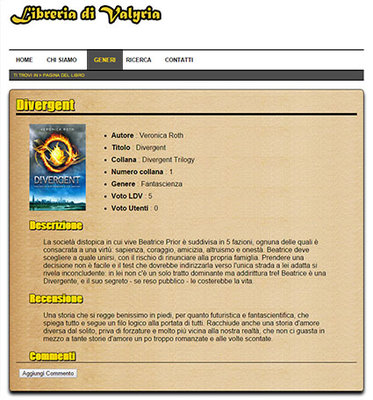
\includegraphics[width=\linewidth]{images/screen/vs_originale.jpg}
\subcaption{Pagina originale (nessun deficit visivo presente)}
\end{minipage}
\hspace{\fill}
\begin{minipage}{0.45\textwidth}
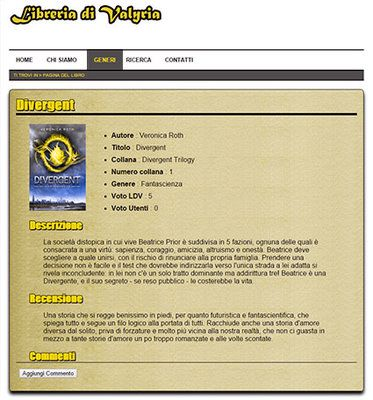
\includegraphics[width=\linewidth]{images/screen/deuteranope.jpg}
\subcaption{Deuteranopia}
\end{minipage}
\vspace*{0.5cm}
\begin{minipage}{0.45\textwidth}
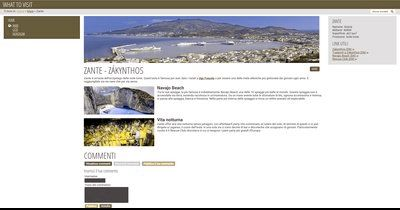
\includegraphics[width=\linewidth]{images/screen/protanope.jpg}
\subcaption{Protanopia}
\end{minipage}
\hspace{\fill}
\begin{minipage}{0.45\textwidth}
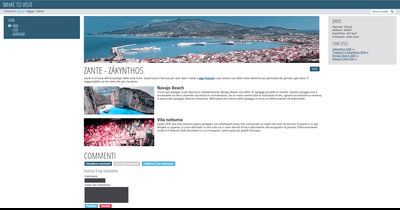
\includegraphics[width=\linewidth]{images/screen/tritanope.jpg}
\subcaption{Tritanopia}
\end{minipage}
\caption{Test con Vischek sulla pagina relativa al singolo libro}\label{multiavp}
\end{figure}

Per quanto riguarda Deuteranopia e Protanopia, la visualizzazione del sito è pressochè identica rispetto all'originale e si differenzia solamente quando si tratta di visualizzare diverse copertine di libri, quando invece si parla di Tritanopia allora si nota un differente modo di vedere gli elementi comuni a tutte le pagine del sito che comunque rimangono accessibili in ogni caso.

\subsection{Visualizzazione in Bianco/Nero}
Abbiamo anche esaminato il sito web con una visualizzazione in scala di grigi notando come alcuni elementi non vengano visualizzati al meglio.

\begin{figure}[H]
\begin{minipage}{0.45\textwidth}
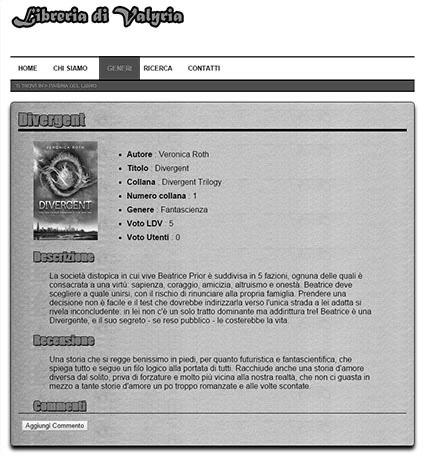
\includegraphics[width=\linewidth]{images/screen/bn_originale.png}
\subcaption{Pagina originale (nessun deficit visivo presente)}
\end{minipage}
\hspace{\fill}
\begin{minipage}{0.45\textwidth}

\includegraphics[width=\linewidth]{images/screen/bn_headerbreadcrumb.jpg}
\subcaption{Header e Breadcrumb}
\end{minipage}
\vspace*{0.5cm}
\begin{minipage}{0.45\textwidth}

\includegraphics[width=\linewidth]{images/screen/bn_tornahome.jpg}
\subcaption{Link Visitato in Accedi.html}
\end{minipage}
\hspace{\fill}
\begin{minipage}{0.45\textwidth}
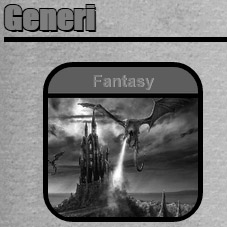
\includegraphics[width=\linewidth]{images/screen/bn_h2etitoli.jpg}
\subcaption{Schede di generi e Titoli}
\end{minipage}
\caption{Errori di visualizzazione nel caso di visione in scala di grigi}\label{multiavp}
\end{figure}

Dalle figure sovrastanti si può notare come vengono visti alcuni elementi quando si effettua una visualizzazione in scala di grigi, e come questi a volte non siano accessibili, come nel caso di link già visitati, in pagine come Accedi o Registrati, Titoli dei Generi, come accade nella pagina di selezione dei generi letterari, o come nel caso di Breadcrumb e Scheda selezionata, in gran parte delle pagine del sito.

\subsection{Fangs}\label{sec:fangs} %DONE
\textit{Fangs} è un'estensione per i browser che consente di visualizzare un
sito nello stesso modo in cui verrebbe visualizzato da uno screen reader,
fornendo il testo come sarebbe letto da questo dispositivo, la lista delle
intestazioni e la lista dei link presenti nella pagina.

In sintesi, come principali problemi vengono individuati:
\begin{itemize}
\item Le parole straniere vengono lette in italiano;
\item A volte i numeri sono scritti in numero; ciò vuol dire che se l'utente
ha la lingua di default del computer/browser impostata su inglese (come nel
caso di un verificatore) si hanno frasi come ``\textit{La società distopica in
cui vive Beatrice Prior è suddivisa in five fazioni}", mentre in casi simili
un numero dovrebbe essere scritto per esteso;
\item Si vedono i nomi dei file delle immagini anzichè un testo alternativo;
\item Quando presente, il testo delle immagini spesso trasmette poca
informazione, ridondando semplicemente il titolo anzichè rimanere vuoto
(soluzione preferibile alla ridondanza);
\item Le abbreviazioni non vengono estese, diventando potenzialmente
incomprensibili.
\end{itemize}

\subsection{Lynx}\label{sec:lynx} %DONE
Le pagine del sito sono state anche navigate tramite il browser testuale
\textit{Lynx}.

Come principale difetto, non è possibile effettuare l'accesso a funzioni come
accesso e registrazione, poichè tutti i pulsanti hanno la sottomissione
dell'input gestita tramite JavaScript, quindi per testare tutte le pagine, si è
provveduto a fare una copia dei file una volta loggati tramite browser e poi
ogni pagina è stata aperta con Lynx.

Gli errori rilevati sono gli stessi discussi nelle altre sezioni.

\subsection{Performance}
Per terminare la fase di testing sono state eseguite, con strumenti
automatici, una serie di verifiche riguardo le performance del sito.

Ci siamo avvalsi di tool online\footnote{\texttt{https://developers.google.com/speed/pagespeed/insights/}, \texttt{http://www.webpagetest.org/},
\texttt{http://gtmetrix.com/}} che analizzano in profondità le pagine HTML
fornite e restituiscono: consigli di ottimizzazione, scale di punteggi per ogni
aspetto del sito e una serie di statistiche che vedremo in dettaglio.\footnote{NB: Per poter utilizzare i tester il sito è stato ``hostato" sulla piattaforma GitHub Pages, come scritto all'inizio di questa sezione}

Al fine di uniformare i risultati raccolti da questi strumenti abbiamo deciso
di mostrare solo alcune delle pagine analizzate, una per ogni livello
gerarchico.
In particolare le più significative per ogni livello (\texttt{homepage.html},
\texttt{citta.html},\texttt{london.html}) hanno dato i seguenti esiti:

\begin{figure}[h]
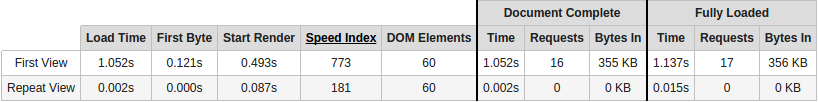
\includegraphics[width=\linewidth]{images/performance/webpagetest/home.png}
\caption{Homepage: tempi di caricamento}
\label{fig:tempiHome}
\end{figure}

\begin{figure}[h]
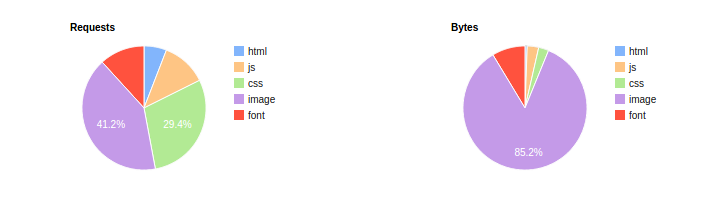
\includegraphics[width=\linewidth]{images/performance/webpagetest/home-graph.png}
\caption{Homepage: Grafico a 'torta' dei tempi di caricamento}
\end{figure}

In homepage si nota la prevalenza del flusso delle immagini, come evidenziato
in fig.\ref{fig:tempiHome}, dal diagramma circolare delle richieste e della
quantità di dati trasmessi dal server.

Come è facile aspettarsi, le immagini occupano in termini di peso la maggior
parte del sito e le richieste per il loro recupero rappresentano più del 40\%
delle richieste totali.


Lo stesso esito è stato conseguito in \texttt{citta.html} e
\texttt{london.html} (fig.\ref{fig:tempiOther}), sebbene \texttt{citta.html}
sia leggermente più pesante dal momento che viene fatto un uso più intenso dei
fogli di stile.

Dopo aver eseguito i test sulle stesse pagine per 3 volte abbiamo stimato che il tempo medio di caricamento complessivo si aggira intorno ai 1400ms.

I test sulla velocità di caricamento sono stati effettuati su di un client residente negli Stati Uniti avente browser Chrome.


\begin{figure}[h]
\begin{minipage}{0.45\textwidth}
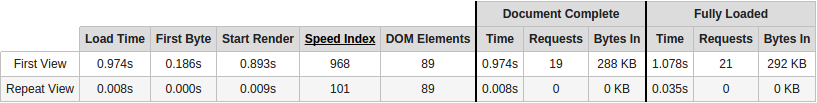
\includegraphics[width=\linewidth]{images/performance/webpagetest/citta.png}
\subcaption{\textit{citta.htm}l: tempi di caricamento}
\end{minipage}
\hspace{\fill}
\vspace*{0.5cm}
\begin{minipage}{0.45\textwidth}

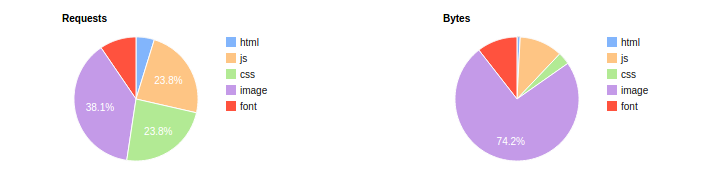
\includegraphics[width=\linewidth]{images/performance/webpagetest/citta-graph.png}
\subcaption{\texttt{citta.html}: grafico a 'torta'}
\end{minipage}

\begin{minipage}{0.45\textwidth}
\vspace*{0.5cm}
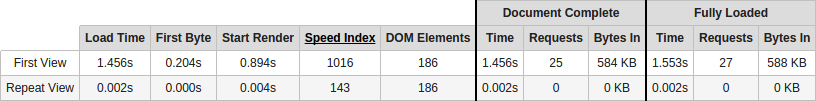
\includegraphics[width=\linewidth]{images/performance/webpagetest/london.png}
\subcaption{\texttt{london.html}: tempi di caricamento}
\end{minipage}
\hspace{\fill}
\vspace*{0.5cm}
\begin{minipage}{0.45\textwidth}

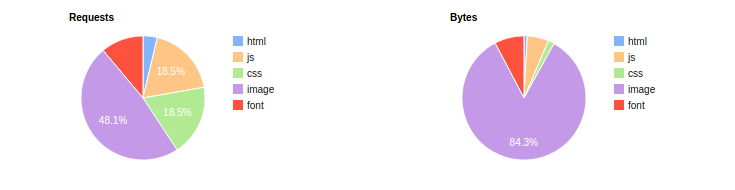
\includegraphics[width=\linewidth]{images/performance/webpagetest/london-graph.png}
\subcaption{\textit{london.html}: grafico a 'torta'}
\end{minipage}
\caption{Performance in \texttt{citta.html} e \texttt{london.html}}\label{multiavp}
\label{fig:tempiOther}
\end{figure}

Complessivamente il sito ha totalizzato una media di 71 punti su 100 totali in Google PageSpeed Insights.

Le ottimizzazioni suggerite per aumentarne il punteggio andavano per lo più
contro standard W3C e/o compatibilità con i browser più obsoleti. Abbiamo
quindi deciso di adottare le soluzioni che permettessero di mantenere
l'accessibilità del sito, cercando di alleggerirlo con piccoli accorgimenti
(e.g. minificazione della libreria Require.js, immagini a risoluzione
inferiore mantenendo una certa qualità di fondo, ecc.) trovando un buon
compromesso tra velocità di caricamento e compatibilità con più browser. % 0%

%%%%%%%%%%%% B====>
%PER NOI: OGNI SEZIONE CHE AGGIUNGETE BASTA METTERLA NELLA CARTELLA sections
%con un certo nome (facciamo finta che sia pippo.tex) E
%POI AGGIUNGERE QUI SOTTO \include{sections\pippo} COME HO FATTO CON L'ABSTRACT
%%%%%%%%%%%% B====>

%----------------------------------------------------------------------------------------

\newpage % Start the article content on the second page, remove this if you have a longer abstract that goes onto the second page

\end{document}

%%%%%%%%%%% B====>
% Dovete stare attenti ad avere installato texlive-full e texlive-publisher (o nome simile)
% Per compilare, make da terminale nella folder dove è contenuto questo file (ho già fatto io il makefile)
% Prima di committare, make clean e cancellare *.pdf
%%%%%%%%%%% B====>
